\documentclass{article}

\usepackage{fancybox,fancyhdr}
\linespread{1.15}
\usepackage{amsfonts}
\usepackage{amsmath}
\usepackage[utf8]{inputenc}
\usepackage[russian]{babel}
\usepackage{hhline}
\usepackage{multirow}
\usepackage{setspace}
\usepackage[usenames]{color}
\usepackage{colortbl}
\usepackage{latexsym}
\usepackage{wasysym}
\usepackage{MnSymbol}

\usepackage{graphicx}  % Для вставки рисунков
\graphicspath{{images/}{images/}}  % папки с картинками
\setlength\fboxsep{3pt} % Отступ рамки \fbox{} от рисунка
\setlength\fboxrule{1pt} % Толщина линий рамки \fbox{}
\usepackage{wrapfig} % Обтекание рисунков и таблиц текстом

\usepackage[usenames,dvipsnames,svgnames,table]{xcolor}
\usepackage{lettrine} %%% To make a Drop Cap
\usepackage{yfonts} %% to make a fancy Gothic drop caps.

\textheight=24.3cm
\textwidth=19cm
\oddsidemargin=-1.2cm
\topmargin=-2cm

\begin{document}

    \pagestyle{fancy}
    \fancyhead{}
    \fancyhead[C]{\normalsize\color{gray}{Коллоквиум определения, 2022 г.}}
    \fancyhead[R]{\normalsize\color{gray}{github.com/Sofiika/AlgebraKollok}}
    \fancyhead[L]{\normalsize\color{gray}{ПИ, линейная алгебра}}
    \fancyfoot[C]{\normalsize\color{gray}{\thepage}}
    \renewcommand{\footrulewidth}{0.1 mm}
    \Large
    \centering

    \textbf{1-й модуль}

    \flushleft
    \small

    \textbf{1. Дать определение умножения матриц. Коммутативна ли эта операция? Ответ пояснить.}


    {
        $\;$
        \setlength{\parindent}{0.4cm}
        \hangindent=0.4cm

    \textit{Произведением матриц} $A_{n\times p}$ и $B_{p\times k}$ называется матрица $C$ типа $n\times k$, где
        $c_{ij}=\sum\limits_{l=1}^p a_{il}\cdot b_{lj}$. Умножение матриц, вообще говоря, не коммутативно, то есть $A\cdot B$, вообще говоря, $\ne B\cdot A$.

        $\;$

        \textbf{Пример:}
        $$
        A=\begin{pmatrix}
              0 & 1 \\
              0 & 0
    \end{pmatrix}, \; B=\begin{pmatrix}
                            0 & 0 \\
                            0 & 1
    \end{pmatrix}
        \qquad
        A\cdot B=\begin{pmatrix}
                     0 & 1 \\
                     0 & 0
    \end{pmatrix}, \; B\cdot A=\begin{pmatrix}
                                   0 & 0 \\
                                   0 & 0
    \end{pmatrix}$$
        $\;$
        \setlength{\parindent}{0cm}
        \hangindent=0cm
    }

    \textbf{2. Дать определение ступенчатого вида матрицы и канонического вида матрицы.}

    {
        $\;$
        \setlength{\parindent}{0.4cm}
        \hangindent=0.4cm

    Матрица $M$ имеет \textit{ступенчатый вид}, если номера первых ненулевых элементов всех строк (такие элементы называют ведущими) возрастают, а нулевые строки стоят внизу матрицы.

        $\;$

        Матрица $M$ имеет \textit{канонический} вид, если $M$ уже имеет ступенчатый вид, причем все ведущие элементы равны 1 и в любом столбце, содержащем ведущий элемент, выше и ниже него стоят 0.

        $\;$
        \setlength{\parindent}{0cm}
        \hangindent=0cm
    }

    \textbf{3. Перечислить элементарные преобразования строк.}

    {
        $\;$
        \setlength{\parindent}{0.4cm}
        \hangindent=0.4cm

    Пусть $(i)$ -- $i$-тая строка матрицы $A$.

    Тогда элементарные преобразования:

    1$\left.\right)$ $(i)\rightarrow\lambda\cdot(i)$, $ \lambda\ne 0$ --
    умножили $i$-тую строку на число $\lambda$

        2$\left.\right)$ $(i)\leftrightarrow (j)$ -- поменяли местами $i$-тую и $j$-тую строки

    3$\left.\right)$ $(i)\rightarrow (i)+\lambda\cdot(k)$ -- $i$-тая строка заменяется на сумму $i$-той строки и $k$-той
    строки $\cdot$ число $\lambda$

        $\;$
        \setlength{\parindent}{0cm}
        \hangindent=0cm
    }

    \textbf{4. Сформулировать теорему о методе Гаусса (алгоритм приводить не нужно).}

    {
        $\;$
        \setlength{\parindent}{0.4cm}
        \hangindent=0.4cm

    Любую конечную матрицу $A$ можно привести элементарными преобразованиями к ступенчатому (каноническому) виду.

        $\;$
        \setlength{\parindent}{0cm}
        \hangindent=0cm
    }

    \textbf{5. Дать определения перестановки и подстановки.}

    {
        $\;$
        \setlength{\parindent}{0.4cm}
        \hangindent=0.4cm

    Всякое расположение чисел от 1 до $n$ в определенном порядке называют \textit{перестановкой}.

        $\;$

        \textit{Подстановка} $\sigma$ {\scriptsize $\begin{pmatrix}
                                                        1         & \ldots & n         \\
                                                        \sigma(1) & \ldots & \sigma(n)
    \end{pmatrix}$} -- отображение множества $1, \ldots, n$ в себя. Это отображение должно быть биективным.

        $\;$
        \setlength{\parindent}{0cm}
        \hangindent=0cm
    }


    \textbf{6. Выписать общую формулу для вычисления определителя произвольного порядка}

    {
        $\;$
        \setlength{\parindent}{0.4cm}
        \hangindent=0.4cm

        $\det A=\sum\limits_{\sigma\in S_n} sgn(\sigma) a_{1\sigma(1)}\cdot a_{2\sigma(2)}\cdot\ldots\cdot a_{n\sigma(n)}$ (сумма по всем подстановкам).

        $\;$
        \setlength{\parindent}{0cm}
        \hangindent=0cm
    }

    \textbf{7. Выписать формулы для разложения определителя по строке и столбцу.}

    {
        $\;$
        \setlength{\parindent}{0.4cm}
        \hangindent=0.4cm

    Определитель матрицы A равен сумме произведений элементов $i$-той строки ($j$-того столбца) на их алгебраические дополнения:
        $$\det A=\sum\limits_{j=1}^n a_{ij}\cdot A_{ij}=\sum\limits_{i=1}^n a_{ij}\cdot A_{ij}$$

        $\;$
        \setlength{\parindent}{0cm}
        \hangindent=0cm
    }

    \newpage

    \textbf{8. Выписать формулы Крамера для квадратной матрицы произвольного порядка.}

    {
        $\;$
        \setlength{\parindent}{0.4cm}
        \hangindent=0.4cm

    Пусть $A\cdot x=b$ -- совместная СЛАУ. Тогда $\triangle_j = x_j\cdot\det(A_1,\ldots, A_n)=\det(A_1, \ldots, A_{j-1}, b, A_{j+1}, \ldots, A_n)$

        Если $\triangle\equiv\det A\ne 0$, то
        $x_j=\frac{\triangle_j}{\triangle}, \; j=\overline{1, n}$\\

        $\;$
        \setlength{\parindent}{0cm}
        \hangindent=0cm
    }




    \textbf{9. Дать определение обратной матрицы. Сформулировать критерий ее существования.}

    {
        $\;$
        \setlength{\parindent}{0.4cm}
        \hangindent=0.4cm

    Матрица $B\in M_n(\mathbb{R})$ называется \textit{обратной} к матрице $A$, если $B\cdot A=E=A\cdot B$.

        $\;$

        Матрица $A\in M_n(\mathbb{R})$ имеет обратную (обратима) $\Leftrightarrow\det A\ne0$ (она невырождена).

        $\;$
        \setlength{\parindent}{0cm}
        \hangindent=0cm
    }

    \textbf{10. Выписать формулу для нахождения обратной матрицы.}

    {
        $\;$
        \setlength{\parindent}{0.4cm}
        \hangindent=0.4cm

        $A^{-1}=\dfrac{1}{\det A}\cdot \tilde A$, где $\tilde A$ -- союзная матрица.

        $\;$
        \setlength{\parindent}{0cm}
        \hangindent=0cm
    }

    \textbf{11. Формула для матрицы обратной к произведению двух матриц}

    {
        $\;$
        \setlength{\parindent}{0.4cm}
        \hangindent=0.4cm

        $(A*B)^{-1} = B^{-1} * A^{-1}$

        $\;$
        \setlength{\parindent}{0cm}
        \hangindent=0cm
    }

    \textbf{12. Дать определение минора.}

    {
        $\;$
        \setlength{\parindent}{0.4cm}
        \hangindent=0.4cm

    Минором $k$-го порядка матрицы $A$ называют определитель матрицы, составленной из элементов, стоящих на пересечениях произвольных $k$ строк и $k$ столбцов.\\

        $\;$
        \setlength{\parindent}{0cm}
        \hangindent=0cm
    }

    \textbf{13. Дать определение базисного минора. Какие строки называются базисными?}

    {
        $\;$
        \setlength{\parindent}{0.4cm}
        \hangindent=0.4cm

    Любой отличный от нуля минор, порядок которого равен рангу, называется \textit{базисным минором} матрицы.

        $\;$

        Строки, попавшие в фиксированный базисный минор, называются \textit{базисными}.

        $\;$
        \setlength{\parindent}{0cm}
        \hangindent=0cm
    }

    \textbf{15. Дать определение линейной комбинации строк. Что такое нетривиальная линейная комбинация?}

    {
        $\;$
        \setlength{\parindent}{0.4cm}
        \hangindent=0.4cm

    \textit{Линейной комбинацией строк (столбцов)} $a_1, \ldots, a_s$ одинаковой длины (высоты) называют выражение вида $\lambda_1\cdot a_1+\ldots+\lambda_s\cdot a_s$, где $\lambda_1, \ldots, \lambda_s$ -- некоторые числа.

        $\;$

        Линейная комбинация называется \textit{нетривиальной}, если $\exists \lambda_i\ne 0$.

        $\;$
        \setlength{\parindent}{0cm}
        \hangindent=0cm
    }

    \textbf{16. Дать определение линейной зависимости строк матрицы.}

    {
        $\;$
        \setlength{\parindent}{0.4cm}
        \hangindent=0.4cm

    Строки $a_1, \ldots, a_s$ называют \textit{линейно зависимыми}, если существует нетривиальная линейная комбинация $\lambda_1\cdot a_1+\ldots+\lambda_s\cdot a_s=0$.

        $\;$
        \setlength{\parindent}{0cm}
        \hangindent=0cm
    }

    \textbf{17. Дать определение линейно независимых столбцов матрицы.}

    {
        $\;$
        \setlength{\parindent}{0.4cm}
        \hangindent=0.4cm

    Если равенство $\lambda_1\cdot a_1+\ldots+\lambda_k\cdot a_k=0$ возможно только при $\lambda_1=\lambda_2=\ldots=\lambda_k=0$, то говорят, что столбцы $a_1, \ldots, a_k$ \textit{линейно независимы} (л.н.з.).

        $\;$
        \setlength{\parindent}{0cm}
        \hangindent=0cm
    }

    \textbf{18. Сформулировать критерий линейной зависимости.}

    {
        $\;$
        \setlength{\parindent}{0.4cm}
        \hangindent=0.4cm

    Строки $a_1, \ldots, a_k$ линейно зависимы $\Leftrightarrow$ хотя бы одна из них является линейной комбинацией остальных.

        $\;$
        \setlength{\parindent}{0cm}
        \hangindent=0cm
    }

    \textbf{19. Сформулировать теорему о базисном миноре.}

    {
        $\;$
        \setlength{\parindent}{0.4cm}
        \hangindent=0.4cm

    1$\left.\right)$ Базисные строки (столбцы), соответсвующие любому базисному минору $M$ матрицы $A$ л.н.з.

    2$\left.\right)$ Строки (столбцы) матрицы $A$, не входящие в $M$, являются линейными комбинациями базисных строк (столбцов).

        $\;$
        \setlength{\parindent}{0cm}
        \hangindent=0cm
    }

    \textbf{20. Сформулировать теорему о ранге матрицы.}

    {
        $\;$
        \setlength{\parindent}{0.4cm}
        \hangindent=0.4cm

    Ранг матрицы равен максимальному числу ее л.н.з. строк (столбцов).

        $\;$
        \setlength{\parindent}{0cm}
        \hangindent=0cm
    }

    \textbf{21. Сформулировать критерий невырожденности квадратной матрицы.}

    {
        $\;$
        \setlength{\parindent}{0.4cm}
        \hangindent=0.4cm

    Рассмотрим матрицу $A\in M_n(\mathbb{R})$. Следующие условия эквивалентны:

    1$\left.\right)$ $\det A\ne 0$

        2$\left.\right)$ $RgA=n$

        3$\left.\right)$ все строки $A$ л.н.з.\\

        $\;$
        \setlength{\parindent}{0cm}
        \hangindent=0cm
    }

    \textbf{22. Сформулируйте теорему Кронекера-Капелли.}

    {
        $\;$
        \setlength{\parindent}{0.4cm}
        \hangindent=0.4cm

    СЛАУ $A\cdot x=b$ совместна $\Leftrightarrow RgA=Rg(A|b)$.

        $\;$
        \setlength{\parindent}{0cm}
        \hangindent=0cm
    }

    \Large
    \centering
    \newpage

    $\;$

    \textbf{2-й модуль}

    \flushleft
    \small


    \textbf{1. Дайте определение фундаментальной системы решений (ФСР) однородной СЛАУ.}

    {
        $\;$
        \setlength{\parindent}{0.4cm}
        \hangindent=0.4cm

    Любые $n-r$ линейно независимых столбцов, являющихся решениями однородной СЛАУ $A\cdot x=0$, где $n$ -- число неизвестных, а $r=RgA$, называют \textit{фундаментальной системой решений} (ФСР) однородной СЛАУ $A\cdot x=0$.

        $\;$
        \setlength{\parindent}{0cm}
        \hangindent=0cm
    }

    \textbf{2. Сформулируйте теорему о структуре общего решения однородной СЛАУ.}

    {
        $\;$
        \setlength{\parindent}{0.4cm}
        \hangindent=0.4cm

    Пусть $\Phi_1, \ldots, \Phi_k$ -- ФСР однородной СЛАУ $A\cdot x=0$. Тогда любое решение этой СЛАУ можно представить в виде
        $x=c_1\cdot\Phi_1+\ldots+c_k\cdot\Phi_k$, где $c_1,\ldots, c_k$ - некоторые постоянные.

        $\;$
        \setlength{\parindent}{0cm}
        \hangindent=0cm
    }

    \textbf{3. Сформулируйте теорему о структуре общего решения неоднородной системы линейных алгебраических уравнений.}

    {
        $\;$
        \setlength{\parindent}{0.4cm}
        \hangindent=0.4cm

    Пусть известно частное решение $\tilde x$ СЛАУ $A\cdot x=b$. Тогда любое решение этой СЛАУ можно
    представить в виде $x=\tilde x+c_1\cdot\Phi_1+\ldots+c_k\cdot\Phi_k$, где $\Phi_1,\ldots, \Phi_k$ -- ФСР соответствующей однородной СЛАУ, а $c_1, \ldots, c_k$ -- некоторые постоянные.

        $\;$
        \setlength{\parindent}{0cm}
        \hangindent=0cm
    }


    \textbf{4. Дайте определение модуля и аргумента комплексного числа. Что такое главное значение аргумента комплексного числа?}

    {
        $\;$
        \setlength{\parindent}{0.4cm}
        \hangindent=0.4cm

    \textit{Модуль комплексного числа} $r=|z|=\sqrt{x^2+y^2}$.

        $\;$

        \textit{Аргумент комплексного числа} -- угол между положительным направлением вещественной оси и радиус-вектором этой точки:
        $$\phi=Arg z=\arg z+2\pi k, \; k\in \mathbb{Z}.$$
        $ \arg z\in[\left. 0, 2\pi\right.) \text{ или} \arg z\in (\left.-\pi, \pi \right. ] - \text{главное значение аргумента}.$

        $\;$
        \setlength{\parindent}{0cm}
        \hangindent=0cm
    }

    \textbf{5. Что происходит с аргументами и модулями комплексных чисел при умножении и делении?}

    {
        $\;$
        \setlength{\parindent}{0.4cm}
        \hangindent=0.4cm


    \textbf{Умножение:} $(x_1, y_1)\cdot(x_2, y_2)=(x_1\cdot x_2-y_1\cdot y_2, x_1\cdot y_2+x_2\cdot y_1)$.

        $\;$

        При умножении модули комплексных чисел перемножаются, а аргументы складываются. Модуль частного двух комплексных чисел равен частному модулей, а аргумент -- разности аргументов делимого и делителя.

        $\;$
        \setlength{\parindent}{0cm}
        \hangindent=0cm
    }


    \textbf{6. Выпишите формулу Муавра.}

    {
        $\;$
        \setlength{\parindent}{0.4cm}
        \hangindent=0.4cm
        $$z^n=r^n(\cos n\phi+i\sin n\phi),\; n\in\mathbb{N}$$

        $\;$
        \setlength{\parindent}{0cm}
        \hangindent=0cm
    }

    \newpage

    \textbf{7. Как найти комплексные корни n-ой степени из комплексного числа? Сделайте эскиз, на котором отметьте исходное число и все корни из него.}

    {
        $\;$
        \setlength{\parindent}{0.4cm}
        \hangindent=0.4cm

    Дано число $w=\rho\cdot(\cos\psi+i\cdot \sin\psi)$ и число $n\in\mathbb{N}$

        $$\sqrt[n]{w}=\left\{z=\sqrt[n]{\rho}\cdot\left(\cos\frac{\psi+2\pi k}{n}+i\cdot\sin\frac{\psi+2\pi k}{n}\right), \; k=\overline{0, n-1}\right\} $$

        $\sqrt[6]{1}:$ \\

    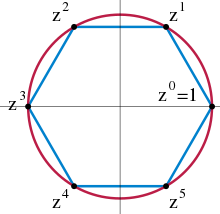
\includegraphics[scale=0.7]{korni2.png}

        $\;$
        \setlength{\parindent}{0cm}
        \hangindent=0cm
    }

    \textbf{8. Сформулируйте основную теорему алгебры. Сформулируйте теорему Безу.}

    {
        $\;$
        \setlength{\parindent}{0.4cm}
        \hangindent=0.4cm

    \textbf{Основная теорема алгебры:} $\forall$ многочлена $f(z)=a_n\cdot z^n+a_{n-1}\cdot z^{n-1}+\ldots+a_0\cdot z^0, \; a_i\in\mathbb{C}, \; n\in\mathbb{N}, \; a_n\ne0$ $\exists$ корень $z_0\in\mathbb{C}$.

        $\;$

        \textbf{Теорема Безу:} Остаток от деления многочлена $f(x)$ на $x-c$ равен $f(c)$.

        $\;$
        \setlength{\parindent}{0cm}
        \hangindent=0cm
    }



    \textbf{9. Какие многочлены называются неприводимыми?}

    {
        $\;$
        \setlength{\parindent}{0.4cm}
        \hangindent=0.4cm

    Многочлен называется \textit{приводимым,} если $\exists$ нетривиальное разложение $f=g\cdot h$ и \textit{неприводимым} в противном случае.

        $\;$
        \setlength{\parindent}{0cm}
        \hangindent=0cm
    }

    \textbf{10. Сформулируйте утверждение о разложении многочленов на неприводимые множители над полем комплексных чисел.}

    {
        $\;$
        \setlength{\parindent}{0.4cm}
        \hangindent=0.4cm

        $\forall$ многочлен степени $n>0$ разлагается в произведение линейных множителей над полем комплексных чисел.

    Комплексный многочлен степени $n$ разлагается в произведение:

        $P_n(z)=a_n\cdot(z-z_1)^{\alpha_1}\cdot \ldots\cdot(z-z_k)^{\alpha_k}$, где сумма кратностей $\alpha_1+\ldots+\alpha_k=n, z_i\in\mathbb{C}$\\

        $\;$
        \setlength{\parindent}{0cm}
        \hangindent=0cm
    }

    \textbf{11. Сформулируйте утверждение о разложении многочленов на неприводимые множители над полем действительных чисел.}

    {
        $\;$
        \setlength{\parindent}{0.4cm}
        \hangindent=0.4cm

        $\forall$ многочлен степени $n>0$ разлагается в произведение линейных множителей и квадратных трехчленов с отрицательным дискриминантом над полем действительных чисел.

    Комплексный многочлен степени $n$ разлагается в произведение:

        $P_n(z)=a_n\cdot(z-z_1)^{\alpha_1}\cdot \ldots\cdot(z-z_k)^{\alpha_k}\cdot(z^2 + p_1 \cdot z + q_1)^{b_1}\cdot\ldots\cdot(z^2 + p_m \cdot z + q_m)^{b_m}$, где сумма кратностей $\alpha_1+\ldots+\alpha_k+b_1+\ldots+b_m=n, z_i\in\mathbb{C}$\\

        $\;$
        \setlength{\parindent}{0cm}
        \hangindent=0cm
    }

    \textbf{12. Дайте определение векторного произведения векторов в трехмерном пространстве.}

    {
        $\;$
        \setlength{\parindent}{0.4cm}
        \hangindent=0.4cm

    Вектор $\overrightarrow{c}$ называют \textit{векторным произведением} векторов $\overrightarrow{a}$ и $\overrightarrow{b}$, если:

    1) $|\overrightarrow{c}|=|\overrightarrow{a}|\cdot|\overrightarrow{b}|\cdot\sin\varphi$, где $\varphi$ - угол между $\overrightarrow{a}$ и $\overrightarrow{b}$

        2) $\overrightarrow{c}\perp\overrightarrow{a}, \overrightarrow{c}\perp\overrightarrow{b}$

        3) тройка $\overrightarrow{a}, \overrightarrow{b}, \overrightarrow{c}$ -- правая

        $\;$
        \setlength{\parindent}{0cm}
        \hangindent=0cm
    }

    \newpage



    \textbf{13. Выпишите формулу для вычисления векторного произведения в координатах, заданных в ортонормированном базисе.}

    {
        $\;$
        \setlength{\parindent}{0.4cm}
        \hangindent=0.4cm

    Пусть $\overrightarrow{i}, \overrightarrow{j}, \overrightarrow{k}$ -- правый ортонормированный базис, $\overrightarrow{a}=a_x\overrightarrow{i}+a_y\overrightarrow{j}+a_z\overrightarrow{k}, \; \overrightarrow{b}=b_x\overrightarrow{i}+b_y\overrightarrow{j}+b_z\overrightarrow{k}$. Тогда: $$\overrightarrow{a}\times\overrightarrow{b}=\begin{vmatrix}
                                                                                                                                                                                                                                                                                                                                                   \overrightarrow{i} & \overrightarrow{j} & \overrightarrow{k} \\
                                                                                                                                                                                                                                                                                                                                                   a_x                & a_y                & a_z                \\
                                                                                                                                                                                                                                                                                                                                                   b_x                & b_y                & b_z
    \end{vmatrix}=\overrightarrow{i}(a_yb_z-b_ya_z)+\overrightarrow{j}(a_zb_x-a_xb_z)+\overrightarrow{k}(a_xb_y-a_yb_x)$$

        $\;$
        \setlength{\parindent}{0cm}
        \hangindent=0cm
    }


    \textbf{14. Что такое уравнение поверхности и его геометрический образ?}

    {
        $\;$
        \setlength{\parindent}{0.4cm}
        \hangindent=0.4cm

    Уравнение $F(x, y, z)=0$ называют \textit{уравнением поверхности} $S$, если этому уравнению удовлетворяют координаты любой точки, лежащей на поверхности, и не удовлетворяют координаты ни одной точки, не лежащей на поверхности.

        $\;$

        При этом поверхность $S$ называют \textit{геометрическим образом} уравнения $F(x, y, z)=0$.

        $\;$
        \setlength{\parindent}{0cm}
        \hangindent=0cm
    }

    \textbf{15. Сформулируйте теорему о том, что задает любое линейное уравнение на координаты точки в трехмерном пространстве.}

    {
        $\;$
        \setlength{\parindent}{0.4cm}
        \hangindent=0.4cm

    Любое уравнение $Ax+By+Cz+D=0$, где $A^2+B^2+C^2>0$, определяет в пространстве плоскость.

        $\;$
        \setlength{\parindent}{0cm}
        \hangindent=0cm
    }

    \textbf{16. Что такое нормаль к плоскости?}

    {
        $\;$
        \setlength{\parindent}{0.4cm}
        \hangindent=0.4cm

    Пусть $Ax+By+Cz+D=0$ -- уравнение плоскости. Тогда вектор $\overrightarrow{n}=(A, B, C)$
        перпендикулярен плоскости и называется нормалью к этой плоскости.

        $\;$
        \setlength{\parindent}{0cm}
        \hangindent=0cm
    }



    \Large
    \centering

    $\;$

    \textbf{3-й модуль}

    \flushleft
    \small

    \textbf{1. Какие бинарные операции называются ассоциативными, а какие коммутативными?}

    {
        $\;$
        \setlength{\parindent}{0.4cm}
        \hangindent=0.4cm

    Бинарная операция $\times$ называется \textit{ассоциативной}, если $\forall a, b, c\in X:$ $a\times(b\times c)=(a\times b)\times c$.

        $\;$

        Бинарная операция $\ast$ называется \textit{коммутативной}, если $\forall a, b\in X$ $a\ast b=b\ast a$.

        $\;$
        \setlength{\parindent}{0cm}
        \hangindent=0cm
    }

    \textbf{2. Дайте определение полугруппы и моноида. Приведите примеры.}

    {
        $\;$
        \setlength{\parindent}{0.4cm}
        \hangindent=0.4cm

    Множество с заданной на нем ассоциативной бинарной операцией называется \textit{полугруппой}. \textbf{Пример:} $(\mathbb{N}, +)$.

        $\;$

        Полугруппа, в которой есть нейтральный элемент, называется \textit{моноидом}. \textbf{Пример:} $(\mathbb{N}, \cdot)$ -- моноид, $e=1$.

        $\;$
        \setlength{\parindent}{0cm}
        \hangindent=0cm
    }

    \textbf{3. Сформулируйте определение группы. Приведите пример.}

    {
        $\;$
        \setlength{\parindent}{0.4cm}
        \hangindent=0.4cm

    Моноид $G$, все элементы которого обратимы, называется \textit{группой}. \textbf{Пример:} множество всех невырожденных $(\det A\ne 0)$ матриц $A_{n\times n}$ с операцией матричного умножения.

        $\;$
        \setlength{\parindent}{0cm}
        \hangindent=0cm
    }

    \textbf{4. Что такое симметрическая группа? Укажите число элементов в ней.}

    {
        $\;$
        \setlength{\parindent}{0.4cm}
        \hangindent=0.4cm

    \textit{Симметрическая группа} $S_n$ -- множество всех подстановок длины $n$ {\scriptsize $\sigma=\begin{pmatrix}
                                                                                                          1   & \ldots & n   \\
                                                                                                          l_1 & \ldots & l_n
    \end{pmatrix}$} с операцией композиции. В ней $n!$ элементов.

        $\;$
        \setlength{\parindent}{0cm}
        \hangindent=0cm
    }

    \newpage

    \textbf{5. Что такое общая линейная и специальная линейная группы?}

    {
        $\;$
        \setlength{\parindent}{0.4cm}
        \hangindent=0.4cm

    Множество всех невырожденных $(\det A\ne 0)$ матриц $A_{n\times n}$ с операцией матричного умножения -- $GL_n(\mathbb{R})$ -- \textit{общая линейная группа}.

        $\;$

        $SL_n(\mathbb{R})=\{A\in GL_n(\mathbb{R})|\det A=1 \}$ -- \textit{специальная линейная группа}.

        $\;$
        \setlength{\parindent}{0cm}
        \hangindent=0cm
    }

    \textbf{6. Сформулируйте определение абелевой группы. Приведите пример.}

    {
        $\;$
        \setlength{\parindent}{0.4cm}
        \hangindent=0.4cm

    Группа с коммутативной операцией называется \textit{абелевой}. \textbf{Пример:} $(\mathbb{Z}, +)$ -- абелева группа.

        $\;$
        \setlength{\parindent}{0cm}
        \hangindent=0cm
    }

    \textbf{7. Дайте определение подгруппы. Приведите пример группы и ее подгруппы.}

    {
        $\;$
        \setlength{\parindent}{0.4cm}
        \hangindent=0.4cm


    Подмножество $H\subseteq G$ называется \textit{подгруппой} в группе $G$, если:

    1) $e\in H$

        2) $\forall h_1, h_2\in H: h_1\cdot h_2\in H$

        3) $\forall h\in H\Rightarrow h^{-1}\in H$

        $\;$

        \textbf{Пример:} $SL_n(\mathbb{R})\subset GL_n(\mathbb{R})$\\

        $\;$
        \setlength{\parindent}{0cm}
        \hangindent=0cm
    }

    \textbf{8. Дайте определение гомоморфизма групп. Приведите пример.}

    {
        $\;$
        \setlength{\parindent}{0.4cm}
        \hangindent=0.4cm


    Отображение $f:G\rightarrow G'$ группы $(G, \ast)$ в группу $(G', \circ)$ называется \textit{гомоморфизмом}, если $\forall a, b\in G$ $f(a\ast b)=f(a)\circ f(b)$.

        $\;$

        \textbf{Пример:} $\det:$ $GL_n(\mathbb{R})\rightarrow\mathbb{R}^{\ast}$ ($\mathbb{R}^{\ast}$ -- это $\mathbb{R}\backslash\{0\}$ с операцией умножения). Это гомоморфизм, так как $\det(A\cdot B)=\det A\cdot \det B$.

        $\;$
        \setlength{\parindent}{0cm}
        \hangindent=0cm
    }

    \textbf{9. Дайте определение изоморфизма групп. Приведите пример.}

    {
        $\;$
        \setlength{\parindent}{0.4cm}
        \hangindent=0.4cm


    \textit{Изоморфизм} -- это биективный гомоморфизм.

        $\;$

        \textbf{Пример:} $(\mathbb{R}, +)\simeq(\mathbb{R}^+, \cdot)$ посредством изоморфизма $f(x)=e^x$.

        $\;$
        \setlength{\parindent}{0cm}
        \hangindent=0cm
    }

    \textbf{10. Дайте определение порядка элемента}

    {
        $\;$
        \setlength{\parindent}{0.4cm}
        \hangindent=0.4cm


    \textit{Порядок элемента} $a\in G$ -- наименьшее натуральное число $p$ такое, что $a^p=e$.

        $\;$
        \setlength{\parindent}{0cm}
        \hangindent=0cm
    }

    \textbf{11. Сформулируйте определение циклической группы. Приведите пример.}

    {
        $\;$
        \setlength{\parindent}{0.4cm}
        \hangindent=0.4cm

    Если $\forall$ элемент $g\in G$ имеет вид $g=a^n=a\times a\times\ldots\times a$ ($n$ раз), где $a\in G$, то $G$ -- \textit{циклическая группа}.

        $\;$

        \textbf{Пример:} $(\mathbb{Z}, +)$ -- циклическая группа, порожденная 1.

        $\;$
        \setlength{\parindent}{0cm}
        \hangindent=0cm
    }

    \textbf{12. Сколько существует, с точностью до изоморфизма, циклических групп данного порядка?}

    {
        $\;$
        \setlength{\parindent}{0.4cm}
        \hangindent=0.4cm

    Существует ровно одна циклическая группа данного порядка с точностью до изоморфизма.

        $\;$
        \setlength{\parindent}{0cm}
        \hangindent=0cm
    }

    \textbf{13. Что такое ядро гомоморфизма групп? Приведите пример.}

    {
        $\;$
        \setlength{\parindent}{0.4cm}
        \hangindent=0.4cm


    \textit{Ядро гомоморфизма} $f:G\rightarrow F$ $Ker f=\{g\in G|f(g)=e_F \}$ ($e_F$ -- нейтральный элелемент в $F$).

        $\;$

        \textbf{Пример:} В гомоморфизме $\mathbb{Z}\rightarrow\mathbb{Z}/3\mathbb{Z}$ с $h(u)=u \mod 3$ ядро состоит из целых чисел, делящихся на 3.

        $\;$
        \setlength{\parindent}{0cm}
        \hangindent=0cm
    }

    \newpage

    \textbf{14. Сформулируйте утверждение о том, какими могут быть подгруппы группы целых чисел по сложению.}

    {
        $\;$
        \setlength{\parindent}{0.4cm}
        \hangindent=0.4cm

        $\forall$ подгруппа в $(\mathbb{Z}, +)$ имеет вид $k\mathbb{Z}$ для некоторых $k\in \mathbb{N}\cup\{0\}$.

        $\;$
        \setlength{\parindent}{0cm}
        \hangindent=0cm
    }

    \textbf{15. Дайте определение левого смежного класса по некоторой подгруппе.}

    {
        $\;$
        \setlength{\parindent}{0.4cm}
        \hangindent=0.4cm

    Пусть $G$ -- группа, $H\subseteq G$ --  подгруппа и $g\in G$. Тогда \textit{левым смежным классом} элемента $g$ по подгруппе $H$ называется множество $gH=\{gh|h\in H \}$.

        $\;$
        \setlength{\parindent}{0cm}
        \hangindent=0cm
    }

    \textbf{16. Дайте определение нормальной подгруппы.}

    {
        $\;$
        \setlength{\parindent}{0.4cm}
        \hangindent=0.4cm

    Подгруппа $H$ называется \textit{нормальной}, если $gH=Hg$, $\forall g\in G$ (равенство правых и левых смежных классов).

        $\;$
        \setlength{\parindent}{0cm}
        \hangindent=0cm
    }

    \textbf{17. Что такое индекс подгруппы?}

    {
        $\;$
        \setlength{\parindent}{0.4cm}
        \hangindent=0.4cm

    \textit{Индексом} подгруппы $H$ в группе $G$ называется число левых смежных классов $G$ по $H$.

        $\;$
        \setlength{\parindent}{0cm}
        \hangindent=0cm
    }

    \textbf{18. Сформулируйте теорему Лагранжа.}

    {
        $\;$
        \setlength{\parindent}{0.4cm}
        \hangindent=0.4cm

    Пусть $G$ -- конечная группа и $H\subseteq G$ -- подгруппа. Тогда $|G|=|H|\cdot[G:H]$.

        $\;$
        \setlength{\parindent}{0cm}
        \hangindent=0cm
    }



    \textbf{19. Сформулируйте три следствия из теоремы Лагранжа.}

    {
        $\;$
        \setlength{\parindent}{0.4cm}
        \hangindent=0.4cm

    \textbf{Следствие 1:} Пусть $G$ -- конечная группа и $g\in G$. Тогда $ord(g)$ делит $|G|$.

        $\;$

        \textbf{Следствие 2:} Пусть $G$ -- конечная группа. Тогда $g^{|G|}=e$.

        $\;$

        \textbf{Следствие 3 (малая теорема Ферма):}
        Пусть $\overline a $ -- ненулевой вычет по простому модулю $p$. Тогда $\overline{a}^{p-1}\equiv1\mod p$.

        $\;$
        \setlength{\parindent}{0cm}
        \hangindent=0cm
    }

    \textbf{20. Сформулируйте критерий нормальности подгруппы, использующий сопряжение.}

    {
        $\;$
        \setlength{\parindent}{0.4cm}
        \hangindent=0.4cm

    Пусть $H\subseteq G$ -- подгруппа в группе $G$. Тогда 3 условия эквивалентны:

    1) $H$ нормальна

    2) $\forall g\in G$ $gHg^{-1}\subseteq H$ ($gHg^{-1}=\{ghg^{-1}|h\in H \}$)

        3) $\forall g\in G$ $gHg^{-1}=H$

        $\;$
        \setlength{\parindent}{0cm}
        \hangindent=0cm
    }

    \textbf{21. Сформулируйте определение простой группы.}

    {
        $\;$
        \setlength{\parindent}{0.4cm}
        \hangindent=0.4cm

    Простая группа - группа, у которой нет подгрупп кроме еденичной и себя самой.

        $\;$
        \setlength{\parindent}{0cm}
        \hangindent=0cm
    }

    \textbf{22. Дайте определение факторгруппы.}

    {
        $\;$
        \setlength{\parindent}{0.4cm}
        \hangindent=0.4cm

    Пусть $H$ -- нормальная подгруппа. Тогда $G/ H$ -- множество левых смежных классов по $H$ с операцией умножения: $(g_1H)\cdot(g_2H)=g_1\cdot g_2H$ называется \textit{факторгруппой} $G$ по $H$.

        $\;$
        \setlength{\parindent}{0cm}
        \hangindent=0cm
    }

    \textbf{23. Что такое естественный гомоморфизм?}

    {
        $\;$
        \setlength{\parindent}{0.4cm}
        \hangindent=0.4cm

    Отображение $\varepsilon:G\rightarrow G/H$, сопоставляющее каждому элементу $a\in G$ его класс смежности $aH$, называется \textit{естественным гомоморфизмом}.

        $\;$
        \setlength{\parindent}{0cm}
        \hangindent=0cm
    }

    \textbf{24. Сформулируйте критерий нормальности подгруппы, использующий понятие ядра гомоморфизма.}

    {
        $\;$
        \setlength{\parindent}{0.4cm}
        \hangindent=0.4cm

        $H$ -- нормальная подгруппа $\Leftrightarrow H=Ker f$, где $f$ -- некоторый гомоморфизм.

        $\;$
        \setlength{\parindent}{0cm}
        \hangindent=0cm
    }

    \textbf{25. Сформулируйте теорему о гомоморфизме групп. Приведите пример.}

    {
        $\;$
        \setlength{\parindent}{0.4cm}
        \hangindent=0.4cm

    Пусть $f:G\rightarrow F$ -- гомоморфизм групп. Тогда группа $Im f =\{a\in F|\exists g\in G, f(g)=a \}$ изоморфна факторгруппе $G/Ker f$, $Ker f=\{g\in G|f(g)=e_F \}$ ($Ker f$ -- ядро гомоморфизма).
        $$G/Ker f\simeq Im f$$

        \textbf{Пример:} $\mathbb{Z}/n\mathbb{Z}\simeq\mathbb{Z}_n$ $f:\mathbb{Z}\rightarrow\mathbb{Z}_n$, $\forall$ целому числу сопоставляем его остаток от деления на $n$ -- $Ker f=n\mathbb{Z}$.

        $\;$
        \setlength{\parindent}{0cm}
        \hangindent=0cm
    }

    \textbf{26. Что такое прямое произведение групп?}

    {
        $\;$
        \setlength{\parindent}{0.4cm}
        \hangindent=0.4cm

    \textit{Прямое произведение групп} $(G, +)\times(D, \star)$ -- это группа из всех пар элементов с операцией поэлементного умножения: $$(g_1, d_1)\times(g_2, d_2)=(g_1+g_2, d_1\star d_2)$$.
        $\;$
        \setlength{\parindent}{0cm}
        \hangindent=0cm
    }

    \textbf{27. Сформулируйте определение автоморфизма и внутреннего автоморфизма.}

    {
        $\;$
        \setlength{\parindent}{0.4cm}
        \hangindent=0.4cm

    \textit{Автоморфизм} -- это изоморфизм из $G$ в $G$.

        $\;$

        \textit{Внутренний автоморфизм} -- это отображение $I_a:g\mapsto aga^{-1}$.

        $\;$
        \setlength{\parindent}{0cm}
        \hangindent=0cm
    }
    \textbf{}\\
    \textbf{}\\
    \textbf{}\\
    \textbf{}\\
    \textbf{28. Что такое центр группы? Что можно сказать о его свойствах? Приведите пример.}

    {
        $\;$
        \setlength{\parindent}{0.4cm}
        \hangindent=0.4cm

    \textit{Центр} группы $G$ -- это множество $Z(G)=\{a\in G|ab=ba\;\forall b\in G \}$. $G$ -- абелева $\Leftrightarrow Z(G)=G$. $Z(G)$ является нормальной подгруппой $G$.

        $\;$
        \setlength{\parindent}{0cm}
        \hangindent=0cm
    }

    \textbf{29. Чему изоморфна факторгруппа группы по ее центру?}

    {
        $\;$
        \setlength{\parindent}{0.4cm}
        \hangindent=0.4cm

        $G/Z(G)\simeq Inn(G)$ ($Inn$ -- подгруппа, которую образуют все внутренние автоморфизмы группы $Aut(G)$).

        $\;$
        \setlength{\parindent}{0cm}
        \hangindent=0cm
    }

    \textbf{30. Сформулируйте теорему Кэли.}

    {
        $\;$
        \setlength{\parindent}{0.4cm}
        \hangindent=0.4cm

        $\forall$ конечная группа порядка $n$ изоморфна некоторой подгруппе группы $S_n$.

        $\;$
        \setlength{\parindent}{0cm}
        \hangindent=0cm
    }

    \textbf{31. Дайте определение кольца.}

    {
        $\;$
        \setlength{\parindent}{0.4cm}
        \hangindent=0.4cm

    Пусть $K\ne \O$ -- множество, на котором заданы две бинарные операции $"+"$ и $"\cdot"$, такие, что:

    1) $(K, +)$ -- абелева группа (это аддитивная группа кольца)

        2) $(K, \cdot)$ -- полугруппа (это мультипликативная полугруппа кольца)

        3) Умножение дистрибутивно относительно сложения: $\forall a, b, c\in K:$ $c(a+b)=ca+cb$, $(a+b)c=ac+bc$

        Тогда $(K, +, \cdot)$ -- \textit{кольцо}.

        $\;$
        \setlength{\parindent}{0cm}
        \hangindent=0cm
    }

    \textbf{32. Что такое коммутативное кольцо? приведите примеры коммутативного и некоммутативного колец.}

    {
        $\;$
        \setlength{\parindent}{0.4cm}
        \hangindent=0.4cm

    Если $\forall x, y\in K\;xy=yx$, то кольцо называется \textit{коммутативным}.

        $\;$

        \textbf{Пример 1:} $(\mathbb{Z}, +, \cdot)$ -- является коммутативным кольцом.

        $\;$

        \textbf{Пример 2:} ($M_n(\mathbb{R}), +, \cdot$) -- полное матричное кольцо над $\mathbb{R}$ -- некоммутативное.

        $\;$
        \setlength{\parindent}{0cm}
        \hangindent=0cm
    }

    \newpage

    \textbf{33. Дайте определение делителей нуля.}

    {
        $\;$
        \setlength{\parindent}{0.4cm}
        \hangindent=0.4cm

    Если $a\cdot b=0$, при $a\ne 0, \; b\ne 0$ в кольце $K$, то $a$ называется \textit{левым делителем нуля}, а $b$ -- \textit{правым делителем нуля}.

        $\;$
        \setlength{\parindent}{0cm}
        \hangindent=0cm
    }



    \textbf{34. Какие элементы кольца называются обратимыми?}

    {
        $\;$
        \setlength{\parindent}{0.4cm}
        \hangindent=0.4cm

    Элемент коммутативного кольца $a$ называется \textit{обратимым}, если $\exists a^{-1}:a\cdot a^{-1}=1=a^{-1}\cdot a$.

        $\;$
        \setlength{\parindent}{0cm}
        \hangindent=0cm
    }

    \textbf{35. Дайте определение поля. Приведите три примера.}

    {
        $\;$
        \setlength{\parindent}{0.4cm}
        \hangindent=0.4cm

    \textit{Поле} $P$ -- это коммутативное кольцо с единицей ($\ne 0$), в котором каждый элемент $a\ne 0$ обратим. \textbf{Пример:} $\mathbb{R}, \mathbb{C}, \mathbb{Q}$.

        $\;$
        \setlength{\parindent}{0cm}
        \hangindent=0cm
    }

    \textbf{36. Дайте определение подполя. Привести пример пары: поле и его подполе.}

    {
        $\;$
        \setlength{\parindent}{0.4cm}
        \hangindent=0.4cm

    \textit{Подполе} -- это подмножество поля, которое само является полем относительно тех же операций. \textbf{Пример:} $\mathbb{Q}\subset\mathbb{R}$.

        $\;$
        \setlength{\parindent}{0cm}
        \hangindent=0cm
    }

    \textbf{37. Дайте определение характеристики поля. Привести примеры: поля конечной положительной характеристики и поля нулевой характеристики.}

    {
        $\;$
        \setlength{\parindent}{0.4cm}
        \hangindent=0.4cm

    Пусть $P$ -- поле. \textit{Характеристикой} поля $P$ ($char P$) называется наименьшее $q\in\mathbb{N}:$ $\underbrace{1+\ldots+1}_{q}=0$. Если такого $q$ не существует, то $char P=0$.

        $\;$

        \textbf{Пример:} $char\mathbb{R}=0$, $char\mathbb{Z}_p=p$, $p$ -- простое.

        $\;$
        \setlength{\parindent}{0cm}
        \hangindent=0cm
    }

    \textbf{38. Сформулируйте утверждение о том, каким будет простое подполе в зависимости от характеристики.}

    {
        $\;$
        \setlength{\parindent}{0.4cm}
        \hangindent=0.4cm

    Пусть $F$ -- поле. $F_0$ -- его простое подполе. Тогда:

    1) если $char F=p>0$, то $F_0\simeq \mathbb{Z}_p$

        2) если $char F=0$, то $F_0\simeq\mathbb{Q}$

        $\;$
        \setlength{\parindent}{0cm}
        \hangindent=0cm
    }

    \textbf{39. Дайте определение идеала. Что такое главный идеал?}

    {
        $\;$
        \setlength{\parindent}{0.4cm}
        \hangindent=0.4cm

    Подмножество $I$ кольца называется \textit{идеалом}, если:

    1. оно является подгруппой по сложению

    2. $\forall a\in I, \forall r\in K\;\; r\cdot a$ и $a\cdot r\in I$

        $\;$

        Идеал называется \textit{главным}, если $\exists a\in K:I=<a>$.

        $\;$
        \setlength{\parindent}{0cm}
        \hangindent=0cm
    }

    \textbf{40. Сформулируйте определение гомоморфизма колец.}

    {
        $\;$
        \setlength{\parindent}{0.4cm}
        \hangindent=0.4cm

        $\varphi:K_1\rightarrow K_2$ -- \textit{гомоморфизм колец}, если $\forall a, b\in K_1:\begin{cases}
                                                                                                  \varphi(a+b)=\varphi(a)\oplus\varphi(b)\\
                                                                                                  \varphi(a\cdot b)=\varphi(a)\ast\varphi(b)
    \end{cases}$

        $\;$
        \setlength{\parindent}{0cm}
        \hangindent=0cm
    }

    \textbf{41. Сформулируйте теорему о гомоморфизме колец. Приведите пример.}

    {
        $\;$
        \setlength{\parindent}{0.4cm}
        \hangindent=0.4cm

    Пусть $\varphi:K_1\rightarrow K_2$ -- гомоморфизм колец. Тогда $K_1/Ker\varphi\simeq Im\varphi$.

        $\;$

        \textbf{Пример:} $\mathbb{Z}/n\mathbb{Z}\simeq\mathbb{Z}_n$ $\varphi:\mathbb{Z}\rightarrow\mathbb{Z}_n$, $\forall$ целому числу сопоставляем его остаток от деления на $n$, $Ker \varphi=n\mathbb{Z}$.

        $\;$
        \setlength{\parindent}{0cm}
        \hangindent=0cm
    }

    \textbf{42. Сформулируйте критерий того, что кольцо вычетов по модулю $p$ является полем.}

    {
        $\;$
        \setlength{\parindent}{0.4cm}
        \hangindent=0.4cm

        $\mathbb{Z}_p$ -- поле $\Leftrightarrow p$ -- простое.

        $\;$
        \setlength{\parindent}{0cm}
        \hangindent=0cm
    }

    \newpage

    \textbf{43. Сформулируйте теорему о том, когда факторкольцо кольца многочленов над полем само является полем.}

    {
        $\;$
        \setlength{\parindent}{0.4cm}
        \hangindent=0.4cm

    Факторкольцо $F[x]/<f(x)>$ является полем $\Leftrightarrow f(x)$ неприводим над $F$.

        $\;$
        \setlength{\parindent}{0cm}
        \hangindent=0cm
    }

    \textbf{44. Дайте определение алгебраического элемента над полем.}

    {
        $\;$
        \setlength{\parindent}{0.4cm}
        \hangindent=0.4cm

    Пусть $F_2$ - поле, а $F_1$ - его подполе. Элемент $\alpha\in F_2$ называется \textit{алгебраическим} над полем $F_1$, если $\exists f(x)\ne0$ (0 как функция), что $f(x)\in F_1[x]$, для которого $f(\alpha)=0$.

        $\;$
        \setlength{\parindent}{0cm}
        \hangindent=0cm
    }



    \textbf{45. Сформулируйте утверждение о том, что любое конечное поле может быть реализовано как факторкольцо кольца многочленов по некоторому идеалу.}

    {
        $\;$
        \setlength{\parindent}{0.4cm}
        \hangindent=0.4cm

        $\forall$ конечное поле $F_q$, где $q=p^n, \;p$ -- простое, можно реализовать в виде $\mathbb{Z}_p[x]/<h(x)>$, где $h(x)$ -- неприводимый многочлен степени $n$ над $\mathbb{Z}_p$.

        $\;$
        \setlength{\parindent}{0cm}
        \hangindent=0cm
    }



    \textbf{46. Дайте определение линейного (векторного) пространства.}

    {
        $\;$
        \setlength{\parindent}{0.4cm}
        \hangindent=0.4cm

    Пусть $F$ -- поле. Пусть $V$ -- произвольное множество, на котором заданы две операции: сложение и умножение на число. Множество $V$ называется \textit{линейным (векторным) пространством}, если $\forall x, y, z\in V, \forall\lambda\mu\in F$ выполнены следующие 8 свойств:

    1) $(x+y)+z=x+(y+z)$ -- ассоциативность сложения

    2) $\exists$ нейтральный элемент по сложению: $\exists 0\in V:\forall x\in V\ x+0=0+x=x$

        3) $\exists$ противоположный элемент по сложению: $\forall x\in V\;\exists(-x)\in V:x+(-x)=0$

        4) $x+y=y+x$ -- коммутативность сложения

    5) $\forall x\in V\quad1\cdot x=x$ -- нейтральность $1\in F$

        6) ассоциативность умножения на число: $\mu(\lambda x)=(\mu\lambda)x$

        7) $(\lambda+\mu)x=\lambda x+\mu x$ -- дистрибутивность относительно умножения на вектор

    8) $\lambda(x+y)=\lambda x+\lambda y$ -- дистрибутивность относительно умножения на число

        $\;$
        \setlength{\parindent}{0cm}
        \hangindent=0cm
    }

    \textbf{47. Дайте определение базиса линейного (векторного) пространства.}

    {
        $\;$
        \setlength{\parindent}{0.4cm}
        \hangindent=0.4cm

    Базисом линейного пространства $V$ называется система векторов $b_1, \ldots, b_n$, такая, что:

    а$\left. \right) $ $b_1, \ldots, b_n$ -- л.н.з.

    б$\left. \right) $ любой вектор из $V$ представляется в виде линейной комбинации $b_1, \ldots, b_n$ $\forall x\in V\;\; x=x_1b_1+\ldots+x_nb_n,\; x_i\in F$

        $\;$
        \setlength{\parindent}{0cm}
        \hangindent=0cm
    }

    \textbf{48. Что такое размерность пространства?}

    {
        $\;$
        \setlength{\parindent}{0.4cm}
        \hangindent=0.4cm

    Максимальное количество л.н.з. векторов в данном линейном пространстве $V$ называется \textit{размерностью пространства} $V$.

        $\;$
        \setlength{\parindent}{0cm}
        \hangindent=0cm
    }

    \textbf{49. Дайте определение матрицы перехода от старого базиса линейного пространства к новому.}

    {
        $\;$
        \setlength{\parindent}{0.4cm}
        \hangindent=0.4cm

    \textit{Матрицей перехода} от базиса $A$ к базису $B$ называется матрица
        \[
            T_{A\rightarrow B}=\begin{pmatrix}
                                   t_{11} & \ldots & t_{1n} \\
                                   \vdots & \ddots & \vdots \\
                                   t_{n1} & \ldots & t_{nn}
            \end{pmatrix}
        \]
        где $t_{1i}, \ldots, t_{ni}$ -- координаты $b_i$ в базисе $A$.

        $\;$
        \setlength{\parindent}{0cm}
        \hangindent=0cm
    }

    \newpage

    \textbf{50. Выпишите формулу для описания изменения координат вектора при изменении базиса.}

    {
        $\;$
        \setlength{\parindent}{0.4cm}
        \hangindent=0.4cm

    Пусть $x\in V, A$ и $B$ -- базисы в $V$. $x^a=\begin{pmatrix}
                                                      x_1^a  \\
                                                      \vdots \\
                                                      x_n^a
    \end{pmatrix}$ -- столбец координат вектора $x$ в базисе $A$,

        $x^b=\begin{pmatrix}
                 x_1^b  \\
                 \vdots \\
                 x_n^b
        \end{pmatrix}$ -- столбец координат вектора $x$ в базисе $B$. Тогда: $$x^b=T_{A\rightarrow B}^{-1}\cdot x^a$$

        $\;$
        \setlength{\parindent}{0cm}
        \hangindent=0cm
    }

    \textbf{51. Дайте определение подпространства в линейном пространстве.}

    {
        $\;$
        \setlength{\parindent}{0.4cm}
        \hangindent=0.4cm

    Подмножество $W$ векторного пространства $V$ называется \textit{подпространством}, если оно само является пространством относительно операций в $V$.

        $\;$
        \setlength{\parindent}{0cm}
        \hangindent=0cm
    }

    \textbf{52. Дайте определения линейной оболочки конечного набора векторов и ранга системы векторов.}

    {
        $\;$
        \setlength{\parindent}{0.4cm}
        \hangindent=0.4cm

    Множество $L(a_1, \ldots, a_k)=\{\lambda_1a_1+\ldots+\lambda_ka_k|\lambda_i\in F \}$ -- множество всех линейных комбинаций векторов $a_1, \ldots, a_k$ называется \textit{линейной оболочкой} системы $a_1, \ldots a_k$

        $\;$

        \textit{Рангом} системы векторов $a_1, \ldots, a_k$ в линейном пространстве называется размерность линейной оболочки этой системы $Rg(a_1, \ldots, a_k)=\dim L(a_1, \ldots a_k)$.

        $\;$
        \setlength{\parindent}{0cm}
        \hangindent=0cm
    }

    \textbf{53. Дайте определения суммы и прямой суммы подпространств.}

    {
        $\;$
        \setlength{\parindent}{0.4cm}
        \hangindent=0.4cm

        $H_1+H_2=\{x_1+x_2|x_1\in H_1, x_2\in H_2 \}$ называется \textit{суммой} подпространств $H_1$ и $H_2$.

        $\;$

        $H_1+H_2$ называется \textit{прямой суммой} (и обзначается $H_1\oplus H_2$), если $H_1\cap H_2=\{0\}$, то есть тривиально.

        $\;$
        \setlength{\parindent}{0cm}
        \hangindent=0cm
    }

    \textbf{54. Сформулируйте утверждение о связи размерности суммы и пересечения подпространств.}

    {
        $\;$
        \setlength{\parindent}{0.4cm}
        \hangindent=0.4cm

    Пусть $H_1$ и $H_2$ -- подпространства. Тогда $\dim(H_1+H_2)=\dim H_1+\dim H_2-\dim(H_1\cap H_2)$.

        $\;$
        \setlength{\parindent}{0cm}
        \hangindent=0cm
    }

    \textbf{55. Дайте определение билинейной формы.}

    {
        $\;$
        \setlength{\parindent}{0.4cm}
        \hangindent=0.4cm

    Функцию $b:V\times V\rightarrow\mathbb{R}$ ($V$ -- линейное пространство над $\mathbb{R}$)  называют \textit{билинейной формой}, если $\forall x, y, z\in V, \;\forall\alpha, \beta\in\mathbb{R}$:

    1) $b(\alpha x+\beta y, z)=\alpha b(x, z)+\beta b(y, z)$

        2) $b(x, \alpha y+\beta z)=\alpha b(x, y)+\beta b(x, z)$

        $\;$
        \setlength{\parindent}{0cm}
        \hangindent=0cm
    }

    \textbf{56. Как меняется матрица билинейной формы при замене базиса?}

    {
        $\;$
        \setlength{\parindent}{0.4cm}
        \hangindent=0.4cm

    Пусть есть базисы $e$ и $e`$. $S$ - матрица перехода от $e$ к $e`$ Тогда билинейная форма $B$ в базисе $e$ равна $B` = S^{T} \cdot B \cdot S$

        $\;$
        \setlength{\parindent}{0cm}
        \hangindent=0cm
    }

    \newpage

    \Large
    \centering

    $\;$

    \textbf{4-й модуль}

    \flushleft
    \small

    \textbf{1. Дайте определение квадратичной формы.}

    {
        $\;$
        \setlength{\parindent}{0.4cm}
        \hangindent=0.4cm

    Однородный многочлен второй степени от $n$ переменных, то есть: $$Q(x)=\sum\limits_{i=1}^n a_{ii}x_i^2+2\sum\limits_{1\leq i<j\leq n} a_{ij}x_ix_j,\; a_{ij}\in\mathbb{R}$$называют \textit{квадратичной формой}.

        $\;$
        \setlength{\parindent}{0cm}
        \hangindent=0cm
    }

    \textbf{2. Дайте определения положительной и отрицательной определенности квадратичной формы.}

    {
        $\;$
        \setlength{\parindent}{0.4cm}
        \hangindent=0.4cm

    Квадратичную форму $Q(x)$ называют:

        \begin{itemize}
            \item \textit{положительно определенной}, если $\forall x\ne 0\ Q(x)>0$
            \item \textit{отрицательно определенной}, если $\forall x\ne 0\ Q(x)<0$\\
        \end{itemize}

        $\;$
        \setlength{\parindent}{0cm}
        \hangindent=0cm
    }



    \textbf{3. Дайте определения канонического и нормального вида квадратичной формы.}

    {
        $\;$
        \setlength{\parindent}{0.4cm}
        \hangindent=0.4cm

    Квадратичную форму $Q(x)=\alpha_1x_1^2+\ldots+\alpha_nx_n^2, \; \alpha_i\in\mathbb{R}\ i=\overline{1, n}$ (то есть не имеющую попарных произведений переменных) называют квадратичной формой \textit{канонического вида}.

        $\;$

        Если $\alpha_i\in\{1, -1, 0\}$, то канонический вид называется \textit{нормальным}.

        $\;$
        \setlength{\parindent}{0cm}
        \hangindent=0cm
    }



    \textbf{4. Сформулируйте критерий Сильвестра и его следствие.}

    {
        $\;$
        \setlength{\parindent}{0.4cm}
        \hangindent=0.4cm

    Квадратичная форма $Q(x)$ от $n$ переменных $x=(x_1, \ldots, x_n)^T$ положительно определена $\Leftrightarrow\begin{cases}
                                                                                                                     \triangle_1>0\\
                                                                                                                     \vdots\\
                                                                                                                     \triangle_n>0
    \end{cases}$. Здесь $Q(x)=x^TAx$, $$A=\begin{pmatrix}
                                              a_{11} & a_{12} & \ldots & a_{1n} \\
                                              a_{21} & a_{22} &        & \vdots \\
                                              \vdots &        & \ddots & \vdots \\
                                              a_{n1} & \ldots & \ldots & a_{nn}
    \end{pmatrix},    \;\triangle_1=a_{11},\; \triangle_2=\begin{vmatrix}
                                                              a_{11} & a_{12} \\
                                                              a_{21} & a_{22}
    \end{vmatrix}, \ldots,\; \triangle_n=\det A$$

        то есть последовательность главных угловых миноров положительна.

        $\;$

        \textbf{Следствие:} $Q(x)$ отрицательно определена $\Leftrightarrow\triangle_1<0, \triangle_2>0, \ldots, (-1)^n\triangle_n>0$ (Знаки главных угловых миноров чередуются, начиная с минуса).

        $\;$
        \setlength{\parindent}{0cm}
        \hangindent=0cm
    }

    \textbf{5. Сформулируйте закон инерции квадратичных форм. Что такое индексы инерции?}

    {
        $\;$
        \setlength{\parindent}{0.4cm}
        \hangindent=0.4cm

    Для любых двух канонических видов одной и той квадратичной формы
        $$Q_1(y_1, \ldots, y_m)=\lambda_1y_1^2+\ldots+\lambda_my_m^2, \lambda_i\ne0, i=\overline{1, m}$$
        $$Q_2(z_1, \ldots, z_k)=\mu_1z_1^2+\ldots+\mu_kz_k^2, \mu_j\ne0, j=\overline{1, k}$$

        $1)\; m=k=RgA$ -- рангу квадратичной формы

    2) количество положительных $\lambda_i=$ количеству положительных $\mu_j=i_+$ -- \textit{положительный индекс инерции}. Количество отрицательных $\lambda_i=$ количеству отрицательных $\mu_j=i_-$ -- \textit{отрицательный индекс инерции}.

        $\;$
        \setlength{\parindent}{0cm}
        \hangindent=0cm
    }

    \newpage

    \textbf{6. Дайте определение линейного отображения. Приведите пример.}

    {
        $\;$
        \setlength{\parindent}{0.4cm}
        \hangindent=0.4cm

    Отображение $\varphi: V_1\rightarrow V_2$ называется \textit{линейным}, если:

    1) $\forall u, v\in V_1, \ \varphi(u+v)=\varphi(u)+\varphi(v)$

        2) $\forall u\in V_1, \forall \lambda\in F\ \varphi(\lambda u)=\lambda\varphi(u)$

        $\;$

        \textbf{Пример:} В линейном пространстве $m\times n$ матриц существует линейное отображение умножения слева на фиксированную матрицу $A_{l\times m}: \varphi:X\rightarrow A\cdot X$.

        $\;$
        \setlength{\parindent}{0cm}
        \hangindent=0cm
    }

    \textbf{7. Дайте определение матрицы линейного отображения.}

    {
        $\;$
        \setlength{\parindent}{0.4cm}
        \hangindent=0.4cm

    \textit{Матрица линейного отображения} -- это матрица $A=\begin{pmatrix}
                                                                 a_{11} & \ldots & a_{1n} \\
                                                                 \vdots & \ddots & \vdots \\
                                                                 a_{m1} & \ldots & a_{mn}
    \end{pmatrix}$, где по столбцам стоят координаты образов векторов базиса $V_1$ в базисе $V_2$.

        $\;$
        \setlength{\parindent}{0cm}
        \hangindent=0cm
    }

    \textbf{8. Выпишите формулу преобразования матрицы линейного отображения при замене базиса. Как выглядит формула в случае линейного оператора?}

    {
        $\;$
        \setlength{\parindent}{0.4cm}
        \hangindent=0.4cm

    Пусть $\varphi$ -- линейное отображение из линейного пространства $V_1$ в линейное пространство $V_2$. Пусть $A_{e_1e_2}$ -- матрица линейного отображения в паре базисов: $e_1$  в пространстве $V_1$ и $e_2$ в пространстве $V_2$ и пусть $T_1$ -- матрица перехода от $e_1$ к $e_1'$, $T_2$ -- матрица перехода от $e_2$ к $e_2'$. Тогда: $$A_{e_1'e_2'}=T_2^{-1}A_{e_1e_2}T_1$$.

    Формула для линейных операторов: $$A_{E'}=T^{-1}A_ET$$

        $\;$
        \setlength{\parindent}{0cm}
        \hangindent=0cm
    }


    \textbf{10. Дайте определения собственного вектора и собственного значения линейного оператора.}

    $\;$
        {
        \setlength{\parindent}{0.4cm}
        \hangindent=0.4cm

        Число $\lambda$ называется \textit{собственным числом} или \textit{собственным значением} линейного оператора $A:V\rightarrow V$, если существует вектор $v\in V, v \not = 0$, такой, что $Av=\lambda v$. При этом вектор $v$ называется \textit{собственным вектором}, отвечающим за собственное значение $\lambda$.

        $\;$
        \setlength{\parindent}{0cm}
        \hangindent=0cm
    }

    \textbf{11. Дайте определения характеристического уравнения и характеристического многочлена квадратной матрицы.}

    $\;$
        {
        \setlength{\parindent}{0.4cm}
        \hangindent=0.4cm

        Для произвольной квадратной матрицы $A$ определитель $\chi_A(\lambda) = \det(A-\lambda E)$ называют \textit{характеристическим многочленом} матрицы $A$. \textit{Характеристическое уравнение} - уравнение вида $\det(A-\lambda E) = 0.$

        $\;$
        \setlength{\parindent}{0cm}
        \hangindent=0cm
    }

    \textbf{12. Сформулируйте утверждение о связи характеристического уравнения и спектра линейного оператора.}

    $\;$
        {
        \setlength{\parindent}{0.4cm}
        \hangindent=0.4cm

        $\lambda$ принадлежит спектру линейного оператора $\Leftrightarrow$ $\lambda$ - корень характеристического уравнения(над алгебраически замкнутым полем).

        $\;$
        \setlength{\parindent}{0cm}
        \hangindent=0cm
    }

    \textbf{13. Дайте определение собственного подпространства.}

    $\;$
        {
        \setlength{\parindent}{0.4cm}
        \hangindent=0.4cm

        Пусть $A:V\rightarrow V$ - линейный оператор, $\lambda$ - собственное значение $A$. Тогда множество $V_\lambda = \{v\in V| Av=\lambda v\}$ - подпространство в $V$, называемое \textit{собственным подпространством}, отвечающим $\lambda$.

        $\;$
        \setlength{\parindent}{0cm}
        \hangindent=0cm
    }

    \newpage

    \textbf{14. Дайте определения алгебраической и геометрической кратности собственного значения. Какое неравенство их связывает?}

    $\;$
        {
        \setlength{\parindent}{0.4cm}
        \hangindent=0.4cm

        \textit{Алгебраической кратностью} $\lambda$ называетсяя кратность $\lambda$ как корня характеристического уравнения. Размерность подпространтсва $V_\lambda$ называется \textit{геометрической кратностью}
        собственного значения $\lambda$. Геометрическая кратность собственного значения не превышает его алгебраической кратности.

        $\;$
        \setlength{\parindent}{0cm}
        \hangindent=0cm
    }


    \textbf{15. Каким свойством обладают собственные векторы линейного оператора, отвечающие различным собственным значениям.}

    $\;$
        {
        \setlength{\parindent}{0.4cm}
        \hangindent=0.4cm

        Пусть $\lambda_1,\dots,\lambda_k$ - собственные значения линейного оператора $A$, $\lambda_i \not = \lambda_j$, а $v_1, \dots, v_k$ - соответствующие собственные векторы. Тогда $v_1, \dots, v_k$ - линейно независимые, т.е. собственные векторы, отвечающие различным собственным значениям, линейно независимы.

        $\;$
        \setlength{\parindent}{0cm}
        \hangindent=0cm
    }

    \textbf{16. Сформулируйте критерий диагональности матрицы оператора.}

    $\;$
        {
        \setlength{\parindent}{0.4cm}
        \hangindent=0.4cm

        Матрица линейного оператора является диагональной в этом базисе $\Leftrightarrow$ все векторы этого базиса являются собственными векторами для $A$.

        $\;$
        \setlength{\parindent}{0cm}
        \hangindent=0cm
    }

    \textbf{17. Сформулируйте критерий диагонализируемости матрицы оператора с использованием понятия геометрической кратности.}

    $\;$
        {
        \setlength{\parindent}{0.4cm}
        \hangindent=0.4cm

        Матрицы линейного оператора приводится к диагональному виду $\Leftrightarrow$ геометрическая кратность каждого собственного значения орператора равна его алгебраической кратности

        $\;$
        \setlength{\parindent}{0cm}
        \hangindent=0cm
    }

    \textbf{18. Дайте определение евклидова пространства.}

    $\;$
        {
        \setlength{\parindent}{0.4cm}
        \hangindent=0.4cm

        \textit{Евклидово пространство} - это пара $V$ - линейное пространство над $\mathbb{R}$ и скалярное произведение $g(x,y)$, то есть симметричная положительно определенная билинейная форма.

        $\;$

        \setlength{\parindent}{0.8cm}
        \hangindent=0.8cm

        $\mathbb{E} = (V, g(x,y))$ и $\forall x, y \in V, \forall \lambda \in \mathbb{R}$:

        \begin{itemize}

            \item  $g(x,y) = g(y,x)$
            \item  $g(x + y, z) = g(x, z) + g(y, z)$
            \item $g(\lambda x, y) = \lambda g(x, y)$
            \item  $g(x, x) \geq 0$ и $ g(x, x) = 0 \Leftrightarrow x= 0$

        \end{itemize}

        \setlength{\parindent}{0.4cm}
        \hangindent=0.4cm

        $\;$
        \setlength{\parindent}{0cm}
        \hangindent=0cm
    }

    \textbf{19. Выпишите неравенство Коши-Буняковского и треугольника.}

    $\;$
        {
        \setlength{\parindent}{0.4cm}
        \hangindent=0.4cm

        Неравенсво Коши-Буняковского: $\forall x, y \in \mathbb{E} \  |(x, y)|\leq||x||\cdot||y||. $

        Неравенсво треугольника: $\forall x, y \in \mathbb{E} \ \Vert x + y \Vert \leq \Vert x \Vert + \Vert y \Vert. $

        $\;$
        \setlength{\parindent}{0cm}
        \hangindent=0cm
    }

    \textbf{20. Дайте определения ортогонального и ортонормированного базисов.}

    $\;$
        {
        \setlength{\parindent}{0.4cm}
        \hangindent=0.4cm

        Пусть $\{v_1, \ldots, v_k \}$ -- ортогональная система векторов, причем $v_i\ne0\ \forall i=\overline{1, k}$.

        Если $k=\dim V=n$, то $v_1, \ldots, v_k$ будут \textit{ортогональным} базисом

        $\;$

        Если рассмотрим $e_1=\dfrac{v_1}{||v_1||}, \ldots, e_n=\dfrac{v_n}{||v_n||}$, то мы получим \textit{ОНБ}\\

        $\;$
        \setlength{\parindent}{0cm}
        \hangindent=0cm
    }

    \newpage

    \textbf{21. Дайте определение матрицы Грама.}

    $\;$
        {
        \setlength{\parindent}{0.4cm}
        \hangindent=0.4cm

        \textit{Матрицей Грама} системы векторов $(e_1, \dots, e_n)$ называется квадратная матрица, состоящая из всевозможных скалярных произведений этих векторов:

        $$
        \Gamma =
        \begin{pmatrix}
        (e_1, e_1)
            & (e_1, e_2) & \dotsb & (e_1, e_n) \\
            (e_2, e_1) & (e_2, e_2) & \dotsb & (e_2, e_n) \\
            \vdots     &            &        & \\
            (e_n, e_1) & (e_n, e_2) & \dotsb & (e_n, e_n)
        \end{pmatrix}
        $$

        $\;$
        \setlength{\parindent}{0cm}
        \hangindent=0cm
    }

    \textbf{23. Выпишите формулу для преобразования матрицы Грама при переходе к новому базису.}

    $\;$
        {
        \setlength{\parindent}{0.4cm}
        \hangindent=0.4cm

        Матрицы Грама двух базисов $e$ и $e'$ связаны соотношением $\Gamma' = U^T \Gamma U $, где $U$ - матрица перехода от $e$ к $e'$.

        $\;$
        \setlength{\parindent}{0cm}
        \hangindent=0cm
    }

    \textbf{25. Сформулируйте критерий линейной зависимости с помощью матрицы Грама.}

    $\;$
        {
        \setlength{\parindent}{0.4cm}
        \hangindent=0.4cm

        Система векторов $e_1, \dots, e_n$
        линейно зависима $\Leftrightarrow$ определитель матрицы Грама этой системы равен нулю.

        $\;$
        \setlength{\parindent}{0cm}
        \hangindent=0cm
    }


    \textbf{26. Дайте определение ортогонального дополнения.}

    $\;$
        {
        \setlength{\parindent}{0.4cm}
        \hangindent=0.4cm

        Пусть $H \subseteq V$. Множество $H^\perp=\{x\in V | (x,y)=0 \; \forall y \in H\}$ называется \textit{ортогональным дополнением}.

        $\;$
        \setlength{\parindent}{0cm}
        \hangindent=0cm
    }

    \textbf{27. Дайте определения ортогональной проекции вектора на подпространство и ортогональной составляющей.}

    {
        $\;$
        \setlength{\parindent}{0.4cm}
        \hangindent=0.4cm

    Пусть $L$ - линейное подпространство евклидова пространства
        $\mathbb{E}$, $a$ - произвольный вектор пространства $\mathbb{E}$. Если $a = b + c$, причём $b \in L, c \in L ^ \perp$, то $b$ называется \textit{ортогональной проекцией} вектора $a$ на
    подпространство $L$ $(proj_La)$, а $c$ - \textit{ортогональной составляющей} при (ортогональном) проектировании вектора a на подпространство $(ort_La)$.

        $\;$
        \setlength{\parindent}{0cm}
        \hangindent=0cm
    }

    \textbf{28. Выпишите формулу для ортогональной проекции вектора на подпространство, заданное как линейная оболочка данного линейно независимого набора векторов.}

    {
        $\;$
        \setlength{\parindent}{0.4cm}
        \hangindent=0.4cm

    Пусть $L=\langle a_1, \dots, a_n \rangle.$ Тогда $proj_L x=A(A^T A)^{-1}A^Tx$, где $A$ - матрица, составленная из столбцов $a_1, \dots, a_n$.

        $\;$
        \setlength{\parindent}{0cm}
        \hangindent=0cm
    }

    \textbf{29. Выпишите формулу для вычисления расстояния с помощью определителей матриц Грама.}

    {
        $\;$
        \setlength{\parindent}{0.4cm}
        \hangindent=0.4cm

    Пусть $S \subset \mathbb{E}$ - подпространство, $x \in \mathbb{E}, (e_1, \dots, e_n)$ - базис $S$. Тогда:

        $$
        (p(x, S))^2 = \frac{\det G(e_1,\dots, e_n, x)}{\det G(e_1, \dots, e_n)}
        $$

        $\;$
        \setlength{\parindent}{0cm}
        \hangindent=0cm
    }

    \textbf{30. Дайте определение сопряженного оператора в евклидовом пространстве.}

    {
        $\;$
        \setlength{\parindent}{0.4cm}
        \hangindent=0.4cm

        Мяу

        $\;$
        \setlength{\parindent}{0cm}
        \hangindent=0cm
    }

    \textbf{31. Дайте определение самосопряженного (симметрического) оператора.}

    {
        $\;$
        \setlength{\parindent}{0.4cm}
        \hangindent=0.4cm

        Мяу

        $\;$
        \setlength{\parindent}{0cm}
        \hangindent=0cm
    }

    \textbf{32. Как найти матрицу сопряженного оператора в произвольном базисе?}

    {
        $\;$
        \setlength{\parindent}{0.4cm}
        \hangindent=0.4cm



        $\;$
        \setlength{\parindent}{0cm}
        \hangindent=0cm
    }

    \textbf{33. Каким свойством обладают собственные значения самосопряженного оператора?}

    {
        $\;$
        \setlength{\parindent}{0.4cm}
        \hangindent=0.4cm

        Мяу

        $\;$
        \setlength{\parindent}{0cm}
        \hangindent=0cm
    }

    \textbf{34. Что можно сказать про собственные векторы самоспоряженного оператора, отвечающие разным собственным значениям?}

    {
        $\;$
        \setlength{\parindent}{0.4cm}
        \hangindent=0.4cm

        Мяу

        $\;$
        \setlength{\parindent}{0cm}
        \hangindent=0cm
    }

    \textbf{35. Сформулируйте определение ортогональной матрицы.}

    {
        $\;$
        \setlength{\parindent}{0.4cm}
        \hangindent=0.4cm

    Матрица $C \in Mat_n(\mathbb{R})$ называется \textit{ортогональной}, если $C^T C = E$.

        $\;$
        \setlength{\parindent}{0cm}
        \hangindent=0cm
    }

    \textbf{36. Дайте определение ортогонального оператора.}

    {
        $\;$
        \setlength{\parindent}{0.4cm}
        \hangindent=0.4cm

    Линейный оператор $\mathcal{A}$ называется \textit{ортогональным}, если $\forall x, y \in \mathbb{E}$ верно, что $(\mathcal{A}x, \mathcal{A}y)= (x, y)$, т.е. оператор сохраняет скалярное произведение, и значит, он сохраняет длины сторон и углы между ними.

        $\;$
        \setlength{\parindent}{0cm}
        \hangindent=0cm
    }


    \textbf{37. Сформулируйте критерий ортогональности оператора, использующий его матрицу.}

    {
        $\;$
        \setlength{\parindent}{0.4cm}
        \hangindent=0.4cm

    Матрица линейного оператора $\mathcal{A}$ в ОНБ ортогональна $\Leftrightarrow$ $\mathcal{A}$ - ортогональный оператор.
        $\;$
        \setlength{\parindent}{0cm}
        \hangindent=0cm
    }

    \textbf{38. Каков канонический вид ортогонального оператора? Сформулируйте теорему Эйлера.}

    {
        $\;$
        \setlength{\parindent}{0.4cm}
        \hangindent=0.4cm

    Для любого отогонального оператора $\mathcal{A}$ существует ортонормированный базис, в котором матрица оператора имеет следующий вид:

        \begin{center}

            $
            \mathcal{A} =
            \begin{pmatrix}
                \Pi(\alpha_1) &        &               &    &        &    &   &        &   \\
                & \ddots &               &    &        &    &   &        &   \\
                &        & \Pi(\alpha_k) &    &        &    &   &        &   \\
                &        &               & -1 &        &    &   &        &   \\
                &        &               &    & \ddots &    &   &        &   \\
                &        &               &    &        & -1 &   &        &   \\
                &        &               &    &        &    & 1 &        &   \\
                &        &               &    &        &    &   & \ddots &   \\
                &        &               &    &        &    &   &        & 1
            \end{pmatrix}
            $ , где $\Pi(\alpha) = \begin{pmatrix}
                                       \cos \alpha & -\sin \alpha \\
                                       \sin \alpha & \cos \alpha
            \end{pmatrix}$

        \end{center}

        $\;$

        \textbf{Теорема Эйлера.} \\
        $\forall$ ортогонального преобразования в $\mathbb{R}^3\ \exists$ ОНБ, в котором его матрица имеет вид$:$

        $A=\begin{pmatrix}
               \cos\varphi & -\sin\varphi & 0    \\
               \sin\varphi & \cos\varphi  & 0    \\
               0           & 0            & \pm1
        \end{pmatrix}$.\\

        $\:$

        \setlength{\parindent}{0cm}
        \hangindent=0cm
    }

    \textbf{39. Сформулируйте теорему о существовании для самосопряженного оператора базиса из собственных векторов.}

    {
        $\;$
        \setlength{\parindent}{0.4cm}
        \hangindent=0.4cm

    Для всякого самосопряженного оператора $\mathcal{A}$ существует ортонормированный базис из собственных векторов, в котором матрица оператора имеет диагональный вид.
        $$\Lambda=diag(\lambda_1,\dots,\lambda_n)$$


        $\lambda_1,\dots,\lambda_n$ - собственные значения оператора $\mathcal{A}$, повторенные в соответствии с их кратностью.

        $\;$
        \setlength{\parindent}{0cm}
        \hangindent=0cm
    }

    \textbf{}

    \textbf{40. Сформулируйте теорему о приведении квадратичной формы к диагональному виду при помощи ортогональной замены координат.}

    {
        $\;$
        \setlength{\parindent}{0.4cm}
        \hangindent=0.4cm

        Мяу

        $\;$
        \setlength{\parindent}{0cm}
        \hangindent=0cm
    }


    \textbf{41. Сформулируйте утверждение о QR-разложении.}

    {
        $\;$
        \setlength{\parindent}{0.4cm}
        \hangindent=0.4cm

    Пусть $A\in M_m(\mathbb{R})$ и столбцы $A_1, \ldots, A_m$ л.н.з. Тогда $\exists\ Q$ и $R:A=QR$, причем $Q$ -- ортогональная матрица,

        $R$ -- верхнетреугольная матрица\\

        $\;$
        \setlength{\parindent}{0cm}
        \hangindent=0cm
    }


    \textbf{42. Сформулируйте теорему о сингулярном разложении.}

    {
        $\;$
        \setlength{\parindent}{0.4cm}
        \hangindent=0.4cm

    Для любой матрицы $A \in Mat_{m \times n}(\mathbb{R})$ существуют ортогональные матрицы $V \in M_m(\mathbb{R})$ и $W \in M_n(\mathbb{R})$ и диагональная матрица $\Sigma \in Mat_{m \times n}(\mathbb{R})$, такие что:

        \begin{center}
            $
            A = V\Sigma W^T
            $, где
            $\Sigma = \left(
            \begin{array}{ccc|ccc}
                \sigma_1 &        &          &   &        &   \\
                & \ddots &          &   & 0      &   \\
                &        & \sigma_r &   &        &   \\
                \hline
                &        &          & 0 &        &   \\
                & 0      &          &   & \ddots &   \\
                &        &          &   &        & 0
            \end{array} \right)
            $ , $\sigma_1 \ge \sigma_2 \ge \ldots \ge \sigma_r > 0$

        \end{center}

        $\;$
        \setlength{\parindent}{0cm}
        \hangindent=0cm
    }


    \textbf{43. Сформулируйте утверждение о полярном разложении.}

    {
        $\;$
        \setlength{\parindent}{0.4cm}
        \hangindent=0.4cm

        $\forall$ матрица $A\in M_n(\mathbb{R})$ представима в виде $A=SU$, где $S$ -- симметрическая матрица с положительными собственными значениями, а $U$ -- ортогональная.\\

        $\;$
        \setlength{\parindent}{0cm}
        \hangindent=0cm
    }

    \textbf{44. Дайте определение сопряженного пространства.}

    {
        $\;$
        \setlength{\parindent}{0.4cm}
        \hangindent=0.4cm

        Мяу

        $\;$
        \setlength{\parindent}{0cm}
        \hangindent=0cm
    }


    \textbf{45. Выпишите формулу для преобразования координат ковектора при переходе к другому базису.}

    {
        $\;$
        \setlength{\parindent}{0.4cm}
        \hangindent=0.4cm

    Пусть $L^*$ - сопряженное пространство. Если записывать координаты элементов по столбцам, то при переходе к другому базису они будут преобразовываться по формуле:
        $$
        [f]_g^{\text{ст}} = T_{e \rightarrow g}^T \cdot [f]_e^{\text{ст}}
        $$

        $\;$
        \setlength{\parindent}{0cm}
        \hangindent=0cm
    }

    \textbf{46. Дайте определение взаимных базисов.}

    {
        $\;$
        \setlength{\parindent}{0.4cm}
        \hangindent=0.4cm

    Базис $\mathfrak{e}=(e_1,\dots,e_n)$ в линейном пространстве $L$ и базис $\mathfrak{f} = (f_1, \dots,f_n)$ в сопряженном пространстве $L^*$ называют \textit{взаимными}, если:
        $$
        (e_i, f^j) = \delta_i^j=\begin{cases}
                                    1, \; i = j \\
                                    0, \; i \not = j
    \end{cases}
        $$

        $\;$
        \setlength{\parindent}{0cm}
        \hangindent=0cm
    }

    \textbf{47. Дайте определение биортогонального базиса.}

    {
        $\;$
        \setlength{\parindent}{0.4cm}
        \hangindent=0.4cm

    Если $L = L^*$, то взаимный к данному базис называется \textit{биортогональным}.

        $\;$
        \setlength{\parindent}{0cm}
        \hangindent=0cm
    }

    \textbf{48. Что можно сказать про ортогональное дополнение к образу сопряженного оператора?}

    {
        $\;$
        \setlength{\parindent}{0.4cm}
        \hangindent=0.4cm

    Пусть линейный оператор $A:E\rightarrow E$. Тогда $E=KerA\oplus ImA^*$\\

        $\;$
        \setlength{\parindent}{0cm}
        \hangindent=0cm
    }


\end{document}
